\documentclass[11pt,letter, swedish, english
]{article}
\pdfoutput=1

\usepackage{../custom_as}
\usepackage[makeroom
]{cancel}
\usepackage{esint}
\let\oldint\int 
\renewcommand{\int}{\oldint\limits}
\graphicspath{{figures/}}

\swapcommands{\Phi}{\varPhi}
\swapcommands{\Omega}{\varOmega}
\swapcommands{\Sigma}{\varSigma}
\swapcommands{\Lambda}{\varLambda}


\newcommand{\enaught}{\ensuremath\varepsilon_0}

%%Drar in tabell och figurtexter
\usepackage[margin=10 pt]{caption}
%%För att lägga in 'att göra'-noteringar i texten
\usepackage{todonotes} %\todo{...}

%%För att själv bestämma marginalerna. 
\usepackage[
%            top    = 2.5cm,
%            bottom = 3cm,
%            left   = 3cm, right  = 3cm
]{geometry}

%%För att ändra hur rubrikerna ska formateras


%\renewcommand{\thefootnote}{\fnsymbol{footnote}}

%\newcommand{\Tc}{\ensuremath{T_{\text{c}}}}
\newcommand{\sign}{\ensuremath{\,\text{sign}}}

%\usepackage{tikz}


\renewcommand{\thesubsection}{\arabic{section} (\alph{subsection})}
\renewcommand{\thesubsubsection}{\arabic{section} (\alph{subsection},\,\roman{subsubsection})}


\begin{document}

%\tikzstyle{every picture}+=[remember picture]
%\tikzstyle{na} = [shape=rectangle,inner sep=0pt,text depth=0pt]



%%%%%%%%%%%%%%%%% vvv Inbyggd titelsida vvv %%%%%%%%%%%%%%%%%

\title{E\&M -- PHYS\,706 \\
Assignment 1}
\author{Andréas Sundström}
\date{\today}

\maketitle

%%%%%%%%%%%%%%%%% ^^^ Inbyggd titelsida ^^^ %%%%%%%%%%%%%%%%%

\section{Electric potential and filed along the $z$ axis}
\begin{figure}\centering
\input{figures/1_geometry.pdf_t}
\caption{The geometry of this problem. Two point charges, each of
  charge $+Q$, are located at $z=\pm R$, and a circular ring centered
  atround the origin with a total charge of $-2Q$.}
\label{fig:1_geometry}
\end{figure}

In this problem, we are tasked to find the electric field and
potential along the $z$~axis, from a geometry given in
\figref{fig:1_geometry}. 

\subsection{The electro static potential}
By the superposition principles we can easili solve this problem in
parts by combining the potentials from each source
$\Phi=\Phi_{+R}+\Phi_{-R}+\Phi_{\text{ring}}$. 

Let's begin with the teo easiest terms. The two terms from the point
charges, which we all know is just
\begin{equation}\label{eq:1_Phi_dot}
\Phi_{\pm{R}}(\vb*r=z\vu{z})=\frac{Q}{4\pi\enaught}
\frac{1}{\abs{\vb*r\mp R\vu{z}}}
=\frac{Q}{4\pi\enaught} \frac{1}{\abs{z\mp R}}.
\end{equation}

Next up is the ring charge. In this case we could easily argue that
the symmetry of the circular charge will make the potential due to
that ring 
\begin{equation}\label{eq:1_Phi_ring}
\Phi_\text{ring}(\vb*r=z\vu{z})=\frac{-2Q}{4\pi\enaught}
\frac{1}{\sqrt{z^2+R^2}},
\end{equation}
where $\sqrt{z^2+R^2}$ is the distance from any point of the ring to
the $z$~axis at $z$. But let's do it more rigorously this time. In
cylindrical coordinates the charge distribution of that ring
is\footnotemark{} 
\begin{equation}
\rho(r, \phi, z)=\lambda \delta(z)\delta(r-R),
\end{equation}
where $\lambda=-2Q/(2\pi R)$ is the uniform linear charge density
along the ring. 
Therefore the potential, at any point in space, due to that ring is
\begin{equation}
\Phi_\text{ring}(y, x, z)=\frac{\lambda}{4\pi\enaught}
\int_0^{2\pi}\rd\phi'\int_{-\infty}^\infty\rd{z'}\int_0^\infty\rd{r'}\,r'
\frac{\delta(z)\delta(r-R)}{\abs{\vb*r-\vb*r'}}
\end{equation}
which upon evaluating the $\delta$ functions yields
\begin{equation}
\Phi_\text{ring}(y, x, z)
= \frac{\lambda}{4\pi\enaught} \int_0^{2\pi}\rd\phi'
\frac{R}{\sqrt{(x-R\cos\phi')^2+(y-R\sin\phi'^2)+z^2}}.
\end{equation}
\footnotetext{I'm using $r$ as the cylindrical radius because $\rho$,
  the more conventional chioce, is already taken for the charge
  density. }

From here, we can clearly see that by setting $x=y=0$ the expression
in the denominator simplifies to $\sqrt{z^2+R^2}$, which is
independent of $\phi'$; we thus end up with exactly
\eqref{eq:1_Phi_ring} as the potential due to the ring on the
$z$~axis.  

The end result from all three sources therefore becomes
\begin{align}\label{eq:1_Phi_a}
\Phi(\vb*r=z\vu{z})=&\frac{Q}{4\pi\enaught}
\qty[\frac{1}{\abs{z-R}}+\frac{1}{\abs{z+R}}
-\frac{2}{\sqrt{z^2+R^2}}]
\\\label{eq:1_Phi_b}
=&\frac{Q}{4\pi\enaught z}
\qty[\frac{1}{\abs{1-R/z}}+\frac{1}{\abs{1+R/z}}
-\frac{2}{\sqrt{1+(R/z)^2}}].
\end{align}

\subsection{The electric field along the $z$ axis}
To calculate the $E$~field along the $z$~axis we use
$\vb*E=-\grad\Phi$, meaning that $E_z=-\pdv*{\Phi}{z}$. This
derivative is easiest done using \eqref{eq:1_Phi_a}. We begin by
rewriting the absolute values\footnotemark, then we differentiate:
\begin{equation}
\begin{aligned}
E_z(\vb*r=z\vu{z})=&
-\frac{Q}{4\pi\enaught} \pdv{z}\qty[
\frac{\sign(z-R)}{(z-R)} +\frac{\sign(z+R)}{(z+R)}
-\frac{2}{\sqrt{z^2+R^2}}]\\
=&-\frac{Q}{4\pi\enaught} \qty[
-\frac{\sign(z-R)}{(z-R)^2} -\frac{\sign(z+R)}{(z+R)^2}
+\frac{2z}{(z^2+R^2)^{3/2}}].
\end{aligned}
\end{equation}
If we want to, we can rewrite this expression as
\begin{equation}
E_z(\vb*r=z\vu{z})
=\frac{Q}{4\pi\enaught z^2} \qty[
\frac{\sign(z-R)}{(1-R/z)^2} +\frac{\sign(z+R)}{(1+R/z)^2}
-\frac{2\sign(z)}{(1+(R/z)^2)^{3/2}}].
\end{equation}
\footnotetext{We are not concerned about the derivatives of the
  ``sign'' functions at their switching point since the rest of the
  expression is not analytic there either. }


\subsection{Asymptotic behaviour of the potential along the $z$ axis}
To find the asymptotic behaviour as $z\to+\infty$, we will need to use
the following Taylor expansion
\begin{equation}
(1+x)^\alpha=1+\alpha x+\frac{\alpha(\alpha-1)}{2}x^2+\order{x^3}
\end{equation}
for sufficiently small $x$. 

In our case, with $\zeta=R/z$, that would correspond to
\begin{equation}
(1\pm\zeta)^{-1}=1\mp\zeta+\zeta^2+\order{\zeta^3}
\end{equation}
and
\begin{equation}
\qty(1+\zeta^2)^{-1/2}=1-\frac{1}{2}\zeta^2+\order{\zeta^4}
\end{equation}
Subsituting these expansions into \eqref{eq:1_Phi_b} gives us the
asymptotic behaviour
\begin{equation}
\Phi(\vb*r=z\vu{z})\sim
\frac{Q}{4\pi\enaught z}
\qty[\qty(1-\zeta+\zeta^2)+\qty(1+\zeta+\zeta^2)
-2\qty(1-\frac{1}{2}\zeta^2)]
=\frac{3Q}{4\pi\enaught}\frac{R^2}{z^3},
\end{equation}
as $\zeta\to0$ or $z\to\infty$.




\section{Charged balls}
\renewcommand{\thesubsection}{\arabic{section} (\roman{subsection})}
This problem concerns charged balls, of radius a, with different chrge
distribution but all with a total charge $Q$. We will be calculating
the $E$-field produced by these charge distributions. 

One generla remark about these fields is that the all have to be of
the form $\vb*E=E_r\vu{r}$, where $\vu{r}$ is the radial unit vector
of a spherical coordinate system. This is due to the spherical
symmetry in this problem. 


\figref{fig:2_e-field} shows a plot of the non-dimensionalized field
strengths as a function of the non-dimensionlized radius
$\xi=r/a$. This is the result of the calculations below. Note that
only the conducting ball produces a discontinuous filed.

\begin{figure}\centering
% GNUPLOT: LaTeX picture with Postscript
\begingroup
  \makeatletter
  \providecommand\color[2][]{%
    \GenericError{(gnuplot) \space\space\space\@spaces}{%
      Package color not loaded in conjunction with
      terminal option `colourtext'%
    }{See the gnuplot documentation for explanation.%
    }{Either use 'blacktext' in gnuplot or load the package
      color.sty in LaTeX.}%
    \renewcommand\color[2][]{}%
  }%
  \providecommand\includegraphics[2][]{%
    \GenericError{(gnuplot) \space\space\space\@spaces}{%
      Package graphicx or graphics not loaded%
    }{See the gnuplot documentation for explanation.%
    }{The gnuplot epslatex terminal needs graphicx.sty or graphics.sty.}%
    \renewcommand\includegraphics[2][]{}%
  }%
  \providecommand\rotatebox[2]{#2}%
  \@ifundefined{ifGPcolor}{%
    \newif\ifGPcolor
    \GPcolortrue
  }{}%
  \@ifundefined{ifGPblacktext}{%
    \newif\ifGPblacktext
    \GPblacktexttrue
  }{}%
  % define a \g@addto@macro without @ in the name:
  \let\gplgaddtomacro\g@addto@macro
  % define empty templates for all commands taking text:
  \gdef\gplbacktext{}%
  \gdef\gplfronttext{}%
  \makeatother
  \ifGPblacktext
    % no textcolor at all
    \def\colorrgb#1{}%
    \def\colorgray#1{}%
  \else
    % gray or color?
    \ifGPcolor
      \def\colorrgb#1{\color[rgb]{#1}}%
      \def\colorgray#1{\color[gray]{#1}}%
      \expandafter\def\csname LTw\endcsname{\color{white}}%
      \expandafter\def\csname LTb\endcsname{\color{black}}%
      \expandafter\def\csname LTa\endcsname{\color{black}}%
      \expandafter\def\csname LT0\endcsname{\color[rgb]{1,0,0}}%
      \expandafter\def\csname LT1\endcsname{\color[rgb]{0,1,0}}%
      \expandafter\def\csname LT2\endcsname{\color[rgb]{0,0,1}}%
      \expandafter\def\csname LT3\endcsname{\color[rgb]{1,0,1}}%
      \expandafter\def\csname LT4\endcsname{\color[rgb]{0,1,1}}%
      \expandafter\def\csname LT5\endcsname{\color[rgb]{1,1,0}}%
      \expandafter\def\csname LT6\endcsname{\color[rgb]{0,0,0}}%
      \expandafter\def\csname LT7\endcsname{\color[rgb]{1,0.3,0}}%
      \expandafter\def\csname LT8\endcsname{\color[rgb]{0.5,0.5,0.5}}%
    \else
      % gray
      \def\colorrgb#1{\color{black}}%
      \def\colorgray#1{\color[gray]{#1}}%
      \expandafter\def\csname LTw\endcsname{\color{white}}%
      \expandafter\def\csname LTb\endcsname{\color{black}}%
      \expandafter\def\csname LTa\endcsname{\color{black}}%
      \expandafter\def\csname LT0\endcsname{\color{black}}%
      \expandafter\def\csname LT1\endcsname{\color{black}}%
      \expandafter\def\csname LT2\endcsname{\color{black}}%
      \expandafter\def\csname LT3\endcsname{\color{black}}%
      \expandafter\def\csname LT4\endcsname{\color{black}}%
      \expandafter\def\csname LT5\endcsname{\color{black}}%
      \expandafter\def\csname LT6\endcsname{\color{black}}%
      \expandafter\def\csname LT7\endcsname{\color{black}}%
      \expandafter\def\csname LT8\endcsname{\color{black}}%
    \fi
  \fi
  \setlength{\unitlength}{0.0500bp}%
  \begin{picture}(7936.00,3968.00)%
    \gplgaddtomacro\gplbacktext{%
      \csname LTb\endcsname%
      \put(860,640){\makebox(0,0)[r]{\strut{} 0}}%
      \put(860,1412){\makebox(0,0)[r]{\strut{} 0.5}}%
      \put(860,2184){\makebox(0,0)[r]{\strut{} 1}}%
      \put(860,2955){\makebox(0,0)[r]{\strut{} 1.5}}%
      \put(860,3727){\makebox(0,0)[r]{\strut{} 2}}%
      \put(980,440){\makebox(0,0){\strut{} 0}}%
      \put(2629,440){\makebox(0,0){\strut{} 0.5}}%
      \put(4278,440){\makebox(0,0){\strut{} 1}}%
      \put(5926,440){\makebox(0,0){\strut{} 1.5}}%
      \put(7575,440){\makebox(0,0){\strut{} 2}}%
      \put(160,2183){\rotatebox{-270}{\makebox(0,0){\strut{}$e(\xi)=E_r(r)\frac{4\pi\enaught a^2}{Q}$}}}%
      \put(4277,140){\makebox(0,0){\strut{}$\xi=(r/a)$}}%
    }%
    \gplgaddtomacro\gplfronttext{%
      \csname LTb\endcsname%
      \put(6792,3514){\makebox(0,0)[r]{\strut{}Conducting ball ($n\to\infty$)}}%
      \csname LTb\endcsname%
      \put(6792,3314){\makebox(0,0)[r]{\strut{}$n=0$}}%
      \csname LTb\endcsname%
      \put(6792,3114){\makebox(0,0)[r]{\strut{}$n=-2$}}%
      \csname LTb\endcsname%
      \put(6792,2914){\makebox(0,0)[r]{\strut{}$n=2$}}%
    }%
    \gplbacktext
    \put(0,0){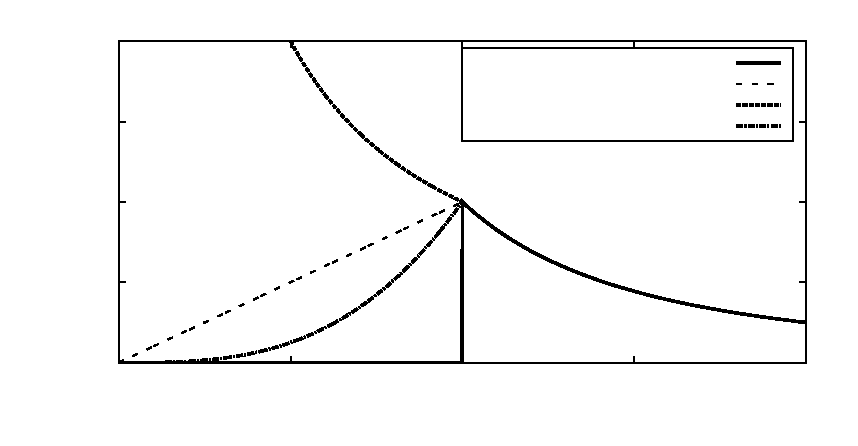
\includegraphics{2_e-field}}%
    \gplfronttext
  \end{picture}%
\endgroup

\caption{A non-dimensionalized plot of some of the electric filed
  strengths produced by the charged balls of radius $\xi=r/a=1$. The first
  graph is the field from a conducting ball, and the three others are
  from balls with charge densities $\rho\propto\xi^n$.}
\label{fig:2_e-field}
\end{figure}

\subsection{Conductive ball}
In this care, we are not explicitly given any chrge distribution, but
we should know by now that all charge on a conductor will gather on
the surface. In other words, there will be no $E$~filed inside the
bulk of the conductor. To show this we can, for instance, use the fact
that $\Phi$ is constant in a conductor; then we 
clearly see that $\vb*E=-\grad\Phi=\vb0$. Furthermore since we have a
ball, the spherical symmetry will result in the charge being evenly
distributed over the surface. 

Now to the field produced by this ball. By applying Gauss's law on
a spherical Gauss surface $S_R$, of radius $R>a$, we get
\begin{equation}
\oiint\limits_{S_R}E_r\vu{r}\vdot\rd\vb*{A}
=\frac{1}{\enaught}\iiint\limits_{V_R} \rho(\vb*r)\id{V}
=\frac{Q}{\enaught}.
\end{equation}
Now since $E_r$ is constant on $S_R$ and $\rd\vb*A=\vu{r}\rd{A}$, the
LHS is just $4\pi R^2\, E_r\!(R)$. The full expression for the $E$~field is
now
\begin{equation}
E_r(r)=
\begin{cases}
0, &r<a,\\
\frac{Q}{4\pi\enaught r^2}\qcomma &r>a,
\end{cases}
\end{equation}
and $\vb*E=E_r\vu{r}$.

We can also note that the field outside any of the balls in this
problem will be the same. This is due to the fact that enclosed charge
by any surface enclosing the whole ball will be~$Q$. 

\subsection{Uniform charge density}
This time we have to use Gauss's law inside the surface as
well. However, the RHS still has the same form. The charge density
will of course be $\rho(r<a)=Q/(4\pi a^3/3)$.
We therefore get
\begin{equation}
4\pi R^2 E_r(R<a)
=\frac{1}{\enaught}\iiint\limits_{V_R}
\frac{3Q}{4\pi a^3}\id{V}
=\frac{Q}{\enaught}\frac{R^3}{a^3}.
\end{equation}
And the final result is
\begin{equation}
E_r(r)=\frac{Q}{4\pi\enaught}\times
\begin{cases}
\frac{r}{a^3}, &r<a,\\
\frac{1}{r^2}\qcomma &r>a.
\end{cases}
\end{equation}

\subsection{Power relation}
In this case we have a power relation for the charge density
$\rho(r<a)\propto r^n$, $n>-3$; i.e. $\rho(r<a)=(r/a)^n\rho_0$. We
have to begin with calculating $\rho_0$. To do this we note that
\begin{equation}\label{eq:2_rho_0}
Q=\iiint\limits_{V_{a}}\rho(r)\id{V}
=\frac{\rho_0}{a^n}\int_0^{2\pi}\rd\phi\int_0^\pi\sin\theta\id\theta
\int_0^a r^n\,r^2\rd{r}
=\frac{4\pi \rho_0}{a^n}\,\frac{a^{n+3}}{n+3}
\end{equation}
so
\begin{equation}
\rho_0=\frac{(n+3)Q}{4\pi a^3}.
\end{equation}

Now to the electric field. We once again use Gauss's law, which will
just be the same integral as in \eqref{eq:2_rho_0} but with 
$a\to R$. So we get
\begin{equation}
4\pi R^2  E_r(R<a)
=\frac{\rho_0}{a^n\enaught}\iiint\limits_{V_R}r^n\id{V}
=\frac{4\pi\rho_0}{a^n\enaught}\,\frac{R^{n+3}}{n+3}
=\frac{Q}{\enaught}\qty(\frac{R}{a})^{n+3},
\end{equation}
and the final electric field will be
\begin{equation}
E_r(r)=\frac{Q}{4\pi\enaught a^2}\times
\begin{cases}
\qty(\frac{r}{a})^{n+1}, &r<a,\\
\qty(\frac{r}{a})^{-2}\qcomma &r>a.
\end{cases}
\end{equation}

Also note that the previous cases just were special cases of this
case. It's easy to see this for the uniform charge distribution, where
$n=0$. But we can reproduce the same behaviour (pointwise) for the
conducting shpere by letting $n\to\infty$.



\section{Mean charge distribution of a hydrogen atom}
\renewcommand{\thesubsection}{\arabic{section} (\alph{subsection})}
Given the mean potential 
\begin{equation}
\Phi(r)=\frac{q}{4\pi\enaught}\,\frac{\ee^{-\alpha r}}{r}
\qty(1+\frac{\alpha r}{2})
\end{equation}
of a neutral hydrogen atom, we now want to find the charge
distribution $\rho(r)$ that would give rise to such a potential.

We begin with the Poisson equation
\begin{equation}
-\laplacian\Phi=\frac{\rho(r)}{\enaught}.
\end{equation}
Then we need to express the Laplacian in spherical coordinates
\begin{equation}
\laplacian f = \frac{1}{r}\pdv[2]{r}[rf] + 
\text{``Derivatives in }\phi\text{ and }\theta\text{''}.
\end{equation}
We only need the $r$ derivatives since we see that $\Phi$ is
spherically symmetric. 

Finding $\rho$ now is just a matter of doing the derivatives
\begin{equation}
\frac{1}{r}\pdv[2]{r}\qty[\ee^{-\alpha r}
\qty(1+\frac{\alpha r}{2})]
=\frac{1}{r} \qty[-\alpha^2\ee^{-\alpha r} 
+\alpha^2\ee^{-\alpha r}\qty(1+\frac{\alpha r}{2})]
=\frac{\alpha^3}{2}\ee^{-\alpha r} 
\end{equation}
So the charge distribution resulting from
this is
\begin{equation}
\rho'(r)=-q\frac{\alpha^3}{8\pi}\ee^{-\alpha r}.
\end{equation}
This would correspond to $-q$ times the electron's probability density
around the nucleus for a ``1s'' state. It is also easy to see that 
\begin{equation}\label{eq:3_q'}
\iiint \rho'(r)\id{V}=-q,
\end{equation}
which means that we have one ``whole'' electron here.

There is one problem thogh; the potential was that of a \emph{neutral}
hydrogen atom. And we can also see that\footnotemark{}
\begin{equation}\label{eq:3_Phi'}
\begin{aligned}
\Phi'(R)&=\frac{1}{4\pi\enaught}\int_0^{2\pi}\rd\phi\int_0^\pi\sin\theta\id\theta
\int_0^\infty\rd{r}\, 
r^2\frac{\rho'(r)}{\sqrt{R^2+r^2-2Rr\cos\theta}}\\
&=\frac{1}{2\enaught}\int_0^\infty\rd{r}\,
\qty(-\frac{q\alpha^3}{8\pi})r^2\ee^{-\alpha r}
\int_0^\pi\frac{\sin\theta\,\rd\theta}{\sqrt{R^2+r^2-2Rr\cos\theta}}\\
\end{aligned}
\end{equation}
To do the $\theta$ integral, we can substitute $u=\cos\theta$ giving
$\rd{u}=-\sin\theta\id\theta$. The $\theta$ integral therefore becomes
\begin{equation}
\begin{aligned}
\int_0^\pi\frac{\sin\theta\,\rd\theta}{\sqrt{R^2+r^2-2Rr\cos\theta}}
=&\int_{-1}^1\frac{\rd{u}}{\sqrt{R^2+r^2-2Rru}}\\
=&-\frac{1}{Rr}\eval{\sqrt{R^2+r^2-2Rru}}_{-1}^1\\
=&\frac{1}{Rr}\Big(|R+r|-|R-r|\Big)
&=\begin{cases}
2/R\qcomma&R>r\\
2/r,&-r<R<r\\
-2/R,&R<-r.
\end{cases}
\end{aligned}
\end{equation}
When we plug this back into \eqref{eq:3_Phi'}, we get
\begin{equation}\label{eq:3_Phi'_final}
\begin{aligned}
\Phi'(R)=&-\frac{q\alpha^3}{16\pi\enaught}\qty{
\int_0^R\frac{2}{R}r^2\ee^{-\alpha r}\id{r}
+\int_R^\infty\frac{2}{r}r^2\ee^{-\alpha r}\id{r} }\\
=&\ldots=-\frac{q}{4\pi\enaught R}
+\frac{q}{4\pi\enaught}\frac{\ee^{-\alpha R}}{R}
\qty(1+\frac{\alpha R}{2}),
\end{aligned}
\end{equation}
which is \emph{not} the potential that we started out with.

\footnotetext{In doing this integral, I've used the common trick of
  setting the ``$z$~axis'' of the spherical integral along the
  direction of the position vector of the field point. This means that
  $|\vb*R-\vb*r|=\sqrt{R^2+r^2-2Rr\cos\theta}$. }


The relatively easy fix here is to insert a $\delta$ function into the
charge distribution:
\begin{equation}
\rho(r)=\rho'(r)+q\delta^3(r).
\end{equation}
It is clear that this will take care of the unwanted term in
\eqref{eq:3_Phi'_final} and the non-zero total charge in
\eqref{eq:3_q'}. 

The reason why we can do this however, is that the Laplacian is
singular at $r=0$; so what we really should have done from the
beginning was to write 
\begin{equation}
\rho(r)=-\enaught\laplacian\Phi+c\delta^3(r),
\end{equation}
and then determined $c$ from the total charge integral. What I did
here was more of a fun(\textinterrobang) exercise.


\section{Capacitances}
This problem concerns the capacitances resulting from some different
geometries. 

We will be using Gauss's law to derive the $E$~filed from the
different geometries. 
\textcolor{gray}{
That usually warrants drawing some figures of
the geometries and suitable Gauss surfaces. The cases in this problem
is however very simple and common (I would guess that they can be
found in any undergraduate E\&M textbook), so I will not bother
drawing anything.
}

\subsection{Plate capacitor}
Here we have two plates, of area $A$, with charge $\pm Q$, separated a
distace $d$ ($d$ is much smaller than any of the sidelengths of the
plates). 

For sufficiently small $d$, we can regard the plates as infinite
whereby the symmetry dictates that, if the plates are parallell to the
$xy$~plane, $\vb*E=E_z\vu{z}$ and allways point away from (into) the
plate if the charge is positive (negative). 

The field from \emph{one} of the plates can therefore be determined by 
\textit{a Gauss surface that is a cylinder with its base parallell and
  mantle perpendicular to the plates}. If the cylinder has a base area
$a$ and the plate has a surface charge density of $\pm\sigma=Q/A$,
then Gauss's law tells us that
\begin{equation}
2a E_z(z)=\frac{a\sigma}{\enaught}
\end{equation}
(assuming that the charge is $+\sigma$).
We get a facor $2a$ on the LHS because we get a contribution of $aE_z(z)$
from each side of the plate. Also note that $E_z(-z)=-E_z(z)$, when
the plate lies in the $z=0$ plane. The field from that one plate is
therefore
\begin{equation}
E_z(z)=\frac{\sigma}{2\enaught}\sign(z).
\end{equation}

The total field inbetween both of these plates is thus
\begin{equation}
E_{z, \text{tot}}(0<z<d)
=\frac{+\sigma}{2\enaught}-\frac{-\sigma}{2\enaught}
=\frac{\sigma}{\enaught},
\end{equation}
(assuming the plate at $z=0$ hade charge $+Q$ and the plate at $z=d$
had $-Q$). The potential difference between these two plates is easily
calculated by doing a \textit{line integral, from the first to the
  second plate, along a straight line perpendicular to the
  plates}. That line integral gives
\begin{equation}
\Delta{V}=\int_0^d\frac{\sigma}{\enaught}\id{z}
=\frac{\sigma d}{\enaught}
=\frac{Qd}{A\enaught}.
\end{equation}
The capacitance is now
\begin{equation}
C=\frac{Q}{\Delta{V}}=\frac{A\enaught}{d}.
\end{equation}


\subsection{Spherical capacitor}
This time we have two concentric spherical shells of radii $a$ and
$b$, where $b>a$. The relevant \textit{Gauss surface here will be
  another concentric sphere of any radius}. The sphereical symmetry of
the geometry results in $\vb*E=E_r\vu{r}$.

We begin by studying the field on the \emph{the inside of the outer
  sphere}. By applying Gauss's law to any sphere inside the puter
shell, we get
\begin{equation}
4\pi r^2 E_{r, \text{outer}}(r<b)=\frac{1}{\enaught}\text{``Enclosed charge''}=0.
\end{equation}
From this we see that the only filed we have inbetween the two shells
will come from the \emph{inner} shell. And by applying Gauss's law to
any shere \emph{outside} that inner shell, we get
\begin{equation}
4\pi r^2 E_{r, \text{inner}}(r>a)=\frac{Q}{\enaught},
\end{equation}
(assuming that the inner sphere has charge $+Q$).

Then the potential difference, which can be calculated with a
\textit{line integral, from the inner to the outer shell, along a
  straight line in the radial direction}. This gives
\begin{equation}
\Delta{V}=\int_a^b\frac{Q}{4\pi\enaught r^2}\id{r}
=\frac{Q}{4\pi\enaught}\qty(\frac{1}{a}-\frac{1}{b})
=\frac{Q}{4\pi\enaught}\qty(\frac{b-a}{ab}).
\end{equation}
And the capacitance is
\begin{equation}
C=\frac{4\pi\enaught ab}{b-a}.
\end{equation}


\subsection{Cylindrical capacitor}
This time it's concentric cylindrical shells of lengths $L$ and radii
$a$ and $b$, where $a<b$. The \textit{Gauss surface is also a
  concentric cylinder}. Once again we can use the symmetry of the
problem to get $\vb*E=E_\rho\vu*\uprho$.

And just like for the spheres, the field from the outer shell will be
$0$ inside the dito. Therefore the only contribution to the potential
difference comes from the inner shell. So let's use Gauss's law on a
Gauss cylinder of length $l\ll L$ and radius $\rho>a$:
\begin{equation}
2\pi\rho l E_\rho(\rho>a)=\frac{\lambda l}{\enaught},
\end{equation}
where $\lambda=Q/L$ (assuming that the inner shell has charge $+Q$).

The potential difference is givn by the \textit{line integral, from the
inner to the outer shell, along any straight line perpendicular to the
$z$~axix}. This gives
\begin{equation}
\Delta{V}=\int_a^b\frac{\lambda}{2\pi\enaught \rho}\id\rho
=\frac{\lambda}{2\pi\enaught}\ln(\frac{b}{a})
=\frac{Q}{2\pi\enaught L}\ln(\frac{b}{a}),
\end{equation}
which gives the capacitance
\begin{equation}\label{eq:3c}
C=\frac{2\pi\enaught L}{\ln(b/a)}.
\end{equation}


\subsection{Application of the previous result}
In this part we will apply the result from the previous part to
calcualte the dimensions of a certain coaxial calbel. The cable has an
outer diameter of $b=\unit[1]{mm}$ and a capacitance of
$c=\unit[3\times10^{-11}]{F/m}$ or $c=\unit[3\times10^{-12}]{F/m}$
($c=C/L$); it is also air filled, meaning that we can use $\enaught$.

From \eqref{eq:3c}, we get
\begin{equation}
\frac{b}{a}=\exp(\frac{2\pi\enaught}{c})
\quad\Longleftrightarrow\quad
a=b\,\exp(-\frac{2\pi\enaught}{c}).
\end{equation}
The two cases we get result in
\begin{equation}
a(c=\unit[3\times10^{-11}]{F/m})=\unit[0.16]{mm}\qcomma
a(c=\unit[3\times10^{-12}]{F/m})=\unit[8.8]{pm}.
\end{equation}
We see that the exponential behaviour makes it practically imposible
to achieve the lower of the two capacitances. 


\subsection*{A quick note on the symmetry of the problem}
I will be using ``the symmetry between $x$ and $y$'' a lot in the
following calculations. By this symmetry I mean that the system is
invariant under the symmetry transformation 
\begin{equation}
[x, y, x_0, y_0] \mapsto [y, x, y_0, y_0].
\end{equation}
I.e. the potential is unchanged under this transformation.




\section{Method of mirrored charges}
\begin{figure}\centering
\input{figures/5_geometry.pdf_t}
\caption{The geometry of probem 5, as seen in the negative $z$
  direction. One line charge, of uniform linear charge density
  $\lambda$, is at $(x_0, y_0)$ perpendicular to the $xy$~plane; then
  there are two grounded planes at $x=0$, $y\ge0$ and at $x\ge0$,
  $y=0$. These planes can be replaced with image charges as drawn in
  this figure (dotted). } 
\label{fig:5_geometry}
\end{figure}

In this problem concerns an infinite line charge perpendicular to the
$xy$ plane, intersecting the plane at  $(x_0, y_0)$ as in
\figref{fig:5_geometry}. There are furthermore two grounded half
planes, parallell to the $z$ axis, cutting off the first quadrant. 

To deal with the two grounded half planes, we will implement the
\emph{method of mirrored charges} (MMC). Let's say that we only had one
grounded plane, for instance the $xz$ plane; then MMC prescribes that
we shuold place an image line charge at $(x_0, -y_0)$. Likewise, if we only
hade the $yz$ plane grounded, then we would need an image line charge
at $(-x_0, y_0)$. This is to ensure that the one plane in the middle
will be at potential $\Phi=0$ due to the symmetry. 

This time, however, we have \emph{two} grounded planes. It is oblious
that just placing out the two image line charges for each plane won't
work. The original charge and one of the image charges will produce
zero potential at the plane inbetween them, but then we would also get
a contribution from the second image charge resulting non-zero
potential on either of the two half planes. 

We therefore need to add one more image charge at $(-x_0, y_0)$. It is
easy to see that this, very symmetric, setup will result in zero
potential on both the $xz$ and $yz$ planes. It is as we had two real
charges at, for instance, $(x_0, \pm{y_0})$ and only the $yz$ plane
was grounded. 


\subsection{The electric potential and field from this geometry}
When we have established the geometry of the images charges, we can
just use the superposition principle to add up the potentials due to
the different charges. One line charge, with linear charge density
$\lambda$, along the $z$ axis will give rise to a potential
\begin{equation}
\Phi_{0,0}(\rho)=\frac{\lambda}{4\pi\enaught}\ln(\frac{a^2}{\rho^2}),
\end{equation}
where $a$ is some constant of dimension length; its contribution
to $\Phi_{0,0}$ is just additive.

So the potential in our case will be
\begin{equation}
\begin{aligned}
\Phi(x, y)=&\Phi_{x_0,y_0}(x, y)-\Phi_{x_0,-y_0}(x, y)
-\Phi_{-x_0,y_0}(x, y)+\Phi_{-x_0,-y_0}(x, y)\\
=&\frac{\lambda}{4\pi\enaught}
\ln(\frac{\qty[(x-x_0)^2+(y+y_0)^2]\qty[(x+x_0)^2+(y-y_0)^2]}
{\qty[(x-x_0)^2+(y-y_0)^2]\qty[(x+x_0)^2+(y+y_0)^2]}).
\end{aligned}
\end{equation}
We aslo see that if we, for instance, set $x=0$ the fraction inside
the log becomes
\begin{equation}
\frac{\bcancel{\qty[x_0^2+(y+y_0)^2]}\cancel{\qty[x_0^2+(y-y_0)^2]}}
{\cancel{\qty[x_0^2+(y-y_0)^2]}\bcancel{\qty[x_0^2+(y+y_0)^2]}}
=1,
\end{equation}
so the potential is indeed $\Phi(x=0, y)=0$; then the symmetry between
$x$ and $y$ means that also $\Phi(x, y=0)=0$.

The tangential $E$ filed at any of the grounded half planes is
calculated using the derivatives in the coordinates parallell to the
plane. Let us look at an example using the $xz$ plane, where we use the $x$
and the $z$ derivatives of $\Phi$. Clearly $\pdv*{\Phi}{z}\equiv0$. So
what we need now is the $x$ derivative. That is more easily calculated
if we split up the logarithms:
\begin{equation}\label{eq:5_ln}
\ln(\frac{\rho_{x_0,-y_0}^2\rho_{-x_0,y_0}^2}
{\rho_{x_0,y_0}^2\rho_{-x_0,-y_0}^2})
=-\ln(\frac{\rho_{x_0,y_0}^2}{a^2})-\ln(\frac{\rho_{-x_0,-y_0}^2}{a^2})
+\ln(\frac{\rho_{x_0,-y_0}^2}{a^2})+\ln(\frac{\rho_{-x_0,y_0}^2}{a^2}),
\end{equation}
where $\rho_{\pm x_0,\pm y_0}^2=(x\mp x_0)^2+(y\mp y_0)^2$. It will
also be helpfull to now that
\begin{equation}
\pdv{(\rho_{\pm x_0,y_0}^2/a^2)}{x}=\frac{2}{a^2}(x\mp x_0)
\end{equation}
Now we can take the $x$ derivative:
\begin{equation}\label{eq:5_dPhi/dx}
\frac{4\pi\enaught}{\lambda}\pdv{\Phi}{x}
=-\frac{2(x-x_0)}{\rho_{x_0,y_0}^2}
-\frac{2(x+x_0)}{\rho_{-x_0,-y_0}^2}
+\frac{2(x-x_0)}{\rho_{x_0,-y_0}^2}
+\frac{2(x+x_0)}{\rho_{-x_0,y_0}^2}.
\end{equation}
Next we set $y=0$. There we note that
\begin{equation}
\rho_{x_0,y_0}(x, y=0)=\rho_{x_0,-y_0}(x, y=0)
\qcomma\text{and}\quad
\rho_{-x_0,y_0}(x=0, y)=\rho_{-x_0,-y_0}(x=0, y).
\end{equation}
Together this results in
\begin{equation}
E_x(x, y=0)=-\eval{\pdv{\Phi}{x}}_{y=0}=0.
\end{equation}

\subsection{Surface charge densities}
In this part of the problem we will calculate the surface charge
density on the grounded half planes. This is easily done since a
surface charge density of $\sigma$ will result in a discontinuity in
the normal $E$~filed of $\sigma/\enaught$. And since the two half
planes are grounded, that means that the $E$~field outside our region
of iterest is 0; i.e. the surface charge density is the same as the
normal $E$~filed just inside the half plane. 

Therefore
\begin{equation}
\frac{1}{\enaught}\sigma_x(x)=E_x(x=0, y)=-\eval{\pdv{\Phi}{x}}_{x=0}.
\end{equation}
Lucky for us, we already calculated the derivative in
\eqref{eq:5_dPhi/dx}. This time, however, we're setting $x=0$, which
means that
\begin{equation}
\rho_{x_0,y_0}(x=0, y)=\rho_{-x_0,y_0}(x=0, y)
\qcomma\text{and}\quad
\rho_{x_0,-y_0}(x=0, y)=\rho_{-x_0,-y_0}(x=0, y).
\end{equation}
The surface charge on the $yz$ plane ($y\ge0$) is therfore
\begin{equation}
\begin{aligned}
\sigma_y(x)=\enaught E_x(x=0, y)=&
\frac{\lambda}{2\pi}
\qty[
\frac{(-x_0)-(x_0)}{x_0^2+(y-y_0)^2}
+\frac{(x_0)-(-x_0)}{x_0^2+(y+y_0)^2}]\\
=&\frac{\lambda x_0}{\pi}
\qty[ \frac{1}{x_0^2+(y+y_0)^2}
-\frac{1}{x_0^2+(y-y_0)^2}].
\end{aligned}
\end{equation}
And, by the symmetry between $x$ and $y$, the surface charge on the
$xz$ plane ($x\ge0$) is therefore
\begin{equation}
\sigma_x(x)=\enaught E_y(x, y=0)=
\frac{\lambda y_0}{\pi}
\qty[
\frac{1}{(x+x_0)^2+y_0^2}
-\frac{1}{(x-x_0)^2+y_0^2}].
\end{equation}

\subsubsection{Plot}
\begin{figure}\centering
% GNUPLOT: LaTeX picture with Postscript
\begingroup
  \makeatletter
  \providecommand\color[2][]{%
    \GenericError{(gnuplot) \space\space\space\@spaces}{%
      Package color not loaded in conjunction with
      terminal option `colourtext'%
    }{See the gnuplot documentation for explanation.%
    }{Either use 'blacktext' in gnuplot or load the package
      color.sty in LaTeX.}%
    \renewcommand\color[2][]{}%
  }%
  \providecommand\includegraphics[2][]{%
    \GenericError{(gnuplot) \space\space\space\@spaces}{%
      Package graphicx or graphics not loaded%
    }{See the gnuplot documentation for explanation.%
    }{The gnuplot epslatex terminal needs graphicx.sty or graphics.sty.}%
    \renewcommand\includegraphics[2][]{}%
  }%
  \providecommand\rotatebox[2]{#2}%
  \@ifundefined{ifGPcolor}{%
    \newif\ifGPcolor
    \GPcolortrue
  }{}%
  \@ifundefined{ifGPblacktext}{%
    \newif\ifGPblacktext
    \GPblacktexttrue
  }{}%
  % define a \g@addto@macro without @ in the name:
  \let\gplgaddtomacro\g@addto@macro
  % define empty templates for all commands taking text:
  \gdef\gplbacktext{}%
  \gdef\gplfronttext{}%
  \makeatother
  \ifGPblacktext
    % no textcolor at all
    \def\colorrgb#1{}%
    \def\colorgray#1{}%
  \else
    % gray or color?
    \ifGPcolor
      \def\colorrgb#1{\color[rgb]{#1}}%
      \def\colorgray#1{\color[gray]{#1}}%
      \expandafter\def\csname LTw\endcsname{\color{white}}%
      \expandafter\def\csname LTb\endcsname{\color{black}}%
      \expandafter\def\csname LTa\endcsname{\color{black}}%
      \expandafter\def\csname LT0\endcsname{\color[rgb]{1,0,0}}%
      \expandafter\def\csname LT1\endcsname{\color[rgb]{0,1,0}}%
      \expandafter\def\csname LT2\endcsname{\color[rgb]{0,0,1}}%
      \expandafter\def\csname LT3\endcsname{\color[rgb]{1,0,1}}%
      \expandafter\def\csname LT4\endcsname{\color[rgb]{0,1,1}}%
      \expandafter\def\csname LT5\endcsname{\color[rgb]{1,1,0}}%
      \expandafter\def\csname LT6\endcsname{\color[rgb]{0,0,0}}%
      \expandafter\def\csname LT7\endcsname{\color[rgb]{1,0.3,0}}%
      \expandafter\def\csname LT8\endcsname{\color[rgb]{0.5,0.5,0.5}}%
    \else
      % gray
      \def\colorrgb#1{\color{black}}%
      \def\colorgray#1{\color[gray]{#1}}%
      \expandafter\def\csname LTw\endcsname{\color{white}}%
      \expandafter\def\csname LTb\endcsname{\color{black}}%
      \expandafter\def\csname LTa\endcsname{\color{black}}%
      \expandafter\def\csname LT0\endcsname{\color{black}}%
      \expandafter\def\csname LT1\endcsname{\color{black}}%
      \expandafter\def\csname LT2\endcsname{\color{black}}%
      \expandafter\def\csname LT3\endcsname{\color{black}}%
      \expandafter\def\csname LT4\endcsname{\color{black}}%
      \expandafter\def\csname LT5\endcsname{\color{black}}%
      \expandafter\def\csname LT6\endcsname{\color{black}}%
      \expandafter\def\csname LT7\endcsname{\color{black}}%
      \expandafter\def\csname LT8\endcsname{\color{black}}%
    \fi
  \fi
  \setlength{\unitlength}{0.0500bp}%
  \begin{picture}(7936.00,3968.00)%
    \gplgaddtomacro\gplbacktext{%
      \csname LTb\endcsname%
      \put(620,949){\makebox(0,0)[r]{\strut{}-4}}%
      \put(620,1566){\makebox(0,0)[r]{\strut{}-2}}%
      \put(620,2184){\makebox(0,0)[r]{\strut{} 0}}%
      \put(620,2801){\makebox(0,0)[r]{\strut{} 2}}%
      \put(620,3418){\makebox(0,0)[r]{\strut{} 4}}%
      \put(740,440){\makebox(0,0){\strut{} 0}}%
      \put(1594,440){\makebox(0,0){\strut{} 0.5}}%
      \put(2449,440){\makebox(0,0){\strut{} 1}}%
      \put(3303,440){\makebox(0,0){\strut{} 1.5}}%
      \put(4158,440){\makebox(0,0){\strut{} 2}}%
      \put(5012,440){\makebox(0,0){\strut{} 2.5}}%
      \put(5866,440){\makebox(0,0){\strut{} 3}}%
      \put(6721,440){\makebox(0,0){\strut{} 3.5}}%
      \put(7575,440){\makebox(0,0){\strut{} 4}}%
      \put(160,2183){\rotatebox{-270}{\makebox(0,0){\strut{}$\Sigma_x(\xi, \theta)$}}}%
      \put(4157,140){\makebox(0,0){\strut{}$\xi$}}%
    }%
    \gplgaddtomacro\gplfronttext{%
      \csname LTb\endcsname%
      \put(6792,3514){\makebox(0,0)[r]{\strut{}$\theta=1/2$}}%
      \csname LTb\endcsname%
      \put(6792,3314){\makebox(0,0)[r]{\strut{}$\theta=1$}}%
      \csname LTb\endcsname%
      \put(6792,3114){\makebox(0,0)[r]{\strut{}$\theta=2$}}%
    }%
    \gplbacktext
    \put(0,0){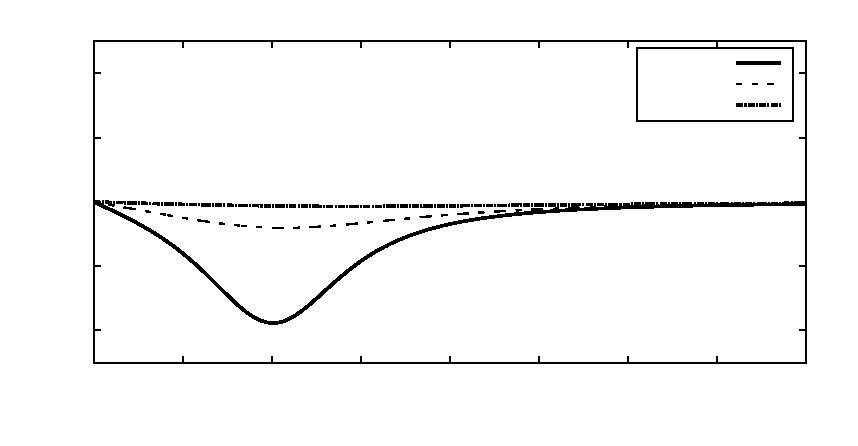
\includegraphics{5_sigma}}%
    \gplfronttext
  \end{picture}%
\endgroup

\caption{Non-dimensionalized surface charge density plotted against
  the non-dimensionalized $x$ coordinate. Here $\Sigma_x$ is given by
  \eqref{eq:5_Sigma_x}, and $\xi=x/x_0$ and $\theta=y_0/x_0$.}
\label{fig:5_sigma}
\end{figure}
We are also tasked with plotting $\sigma_x(x)$ again $x$, for some
different values of $x_0$ and $y_0$. In a case like this, what we
should really do is plot two \emph{dimension-less} quantities against
each other. So instead of $\sigma_x$ versus $x$, we can use
\begin{equation}\label{eq:5_Sigma_x}
\Sigma_x(\xi, \theta)=\frac{\pi \sigma_x x_0^2}{\lambda y_0}
=\frac{1}{(1+\xi)^2+\theta^2}-\frac{1}{(1-\xi)^2+\theta^2},
\end{equation}
where $\xi=x/x_0$ and $\theta=y_0/x_0$.

The plots using these variables are shown in \figref{fig:5_sigma}. We
clearly see that the closer the line charge is to the plane (compared
to the other plane), the stronger the surface charge density becomes. 

\subsection{Total charge on the plane}
To get the total charge per unit length, in the $z$ direction, of the
$xz$~plane ($x\ge0$) we just integrate over the positive $x$~axis:
\begin{equation}
\begin{aligned}
\Lambda_x=&\int_0^\infty\rd{x}\,\sigma_x(x)
=\int_0^\infty x_0\rd{\xi}\,\frac{\lambda y_0}{\pi x_0^2}
\qty[\frac{1}{(1+\xi)^2+\theta^2}-\frac{1}{(1-\xi)^2+\theta^2}]\\
=&\frac{\lambda \theta}{\pi}
\int_0^\infty \rd{\xi}\,\frac{1}{\theta^2}
\qty[\frac{1}{(1+\xi)^2/\theta^2+1}-\frac{1}{(1-\xi)^2/\theta^2+1}].
\end{aligned}
\end{equation}
From here, we can spit this integral into two separate integral with
the new variabels
\begin{equation}
u_\pm=\frac{\xi\pm1}{\theta}
\quad\Longrightarrow\quad
\rd\xi=\theta\id{u_\pm}.
\end{equation}
And we get
\begin{equation}
\begin{aligned}
\Lambda_x=&\frac{\lambda}{\pi}
\qty[\;\int_{1/\theta}^\infty \frac{\rd u_+}{u_+^2+1}
-\int_{-1/\theta}^\infty\frac{\rd u_-}{u_-^2+1}\;]\\
=&\frac{\lambda}{\pi}\qty{
\qty[\frac{\pi}{2}-\arctan(\theta^{-1})]
-\qty[\frac{\pi}{2}-\arctan(-\theta^{-1})]}\\
=&-\frac{2\lambda}{\pi}\arctan(\theta^{-1})
&=-\frac{2\lambda}{\pi}\arctan(\frac{x_0}{y_0}).
\end{aligned}
\end{equation}
By the symmetry between $x$ and $y$ in this problem, we also have
\begin{equation}
\Lambda_y=-\frac{2\lambda}{\pi}\arctan(\frac{y_0}{x_0}).
\end{equation}


\subsection{Asymptotic behavior}
To calculate the asymptotic behaviour it will be helpfull to know
the distance between two points $\vb*r'$ and $\vb*r$, in cylidrical
coordimnates. Assumin that $\vb*r'$ has cyulidrical coordinates
$(\rho', \phi')$ and similar for $\vb*r$, we get
\begin{equation}
|\vb*r-\vb*r'|^2=\rho^2+{\rho'}^2-2\rho\rho'\cos(\phi-\phi').
\end{equation}

Next up we note that the four charges have cylindrical coordinate
angles $\pm\phi_0$ or $\pi\pm\phi_0$, but all have radius $\rho_0$.
This means that we can rewrite the logarithms on the RHS of
\eqref{eq:5_ln} as
\begin{equation}
\begin{aligned}
\text{RHS\eqref{eq:5_ln}}=&
-\ln(\frac{\rho^2}{a^2}
  \qty[1+\frac{\rho_0^2}{\rho^2}-2\frac{\rho_0}{\rho}\cos(\phi-\phi_0)])
-\ln(\frac{\rho^2}{a^2}
  \qty[1+\frac{\rho_0^2}{\rho^2}-2\frac{\rho_0}{\rho}\cos(\phi-(\pi+\phi_0))])\\
&+\ln(\frac{\rho^2}{a^2}
  \qty[1+\frac{\rho_0^2}{\rho^2}-2\frac{\rho_0}{\rho}\cos(\phi+\phi_0)])
+\ln(\frac{\rho^2}{a^2}
  \qty[1+\frac{\rho_0^2}{\rho^2}-2\frac{\rho_0}{\rho}\cos(\phi-(\pi-\phi_0))])\\
=&
-\ln(1+\frac{\rho_0^2}{\rho^2}-2\frac{\rho_0}{\rho}\cos(\phi-\phi_0))
-\ln(1+\frac{\rho_0^2}{\rho^2}+2\frac{\rho_0}{\rho}\cos(\phi-\phi_0))\\
&+\ln(1+\frac{\rho_0^2}{\rho^2}-2\frac{\rho_0}{\rho}\cos(\phi+\phi_0))
+\ln(1+\frac{\rho_0^2}{\rho^2}+2\frac{\rho_0}{\rho}\cos(\phi+\phi_0)).
\end{aligned}
\end{equation}
Now we want to investigate the behavior as $\rho\to\infty$ or
$\epsilon=\rho_0/\rho\to0$. 
\begin{equation}
\begin{aligned}
\text{RHS\eqref{eq:5_ln}}=&
-\ln(1+\epsilon^2-2\epsilon\cos(\phi-\phi_0))
-\ln(1+\epsilon^2+2\epsilon\cos(\phi-\phi_0))\\
&+\ln(1+\epsilon^2-2\epsilon\cos(\phi+\phi_0))
+\ln(1+\epsilon^2+2\epsilon\cos(\phi+\phi_0))\\
=&-\qty[\qty(\xcancel{\epsilon^2}-\cancel{2\epsilon\cos(\phi-\phi_0)})
-\frac{1}{2}\qty(\epsilon^2-2\epsilon\cos(\phi-\phi_0))^2]\\
&-\qty[\qty(\xcancel{\epsilon^2}+\cancel{2\epsilon\cos(\phi-\phi_0)})
-\frac{1}{2}\qty(\epsilon^2+2\epsilon\cos(\phi-\phi_0))^2]\\
&+\qty[\qty(\xcancel{\epsilon^2}-\bcancel{2\epsilon\cos(\phi+\phi_0)})
-\frac{1}{2}\qty(\epsilon^2-2\epsilon\cos(\phi+\phi_0))^2]\\
&+\qty[\qty(\xcancel{\epsilon^2}+\bcancel{2\epsilon\cos(\phi+\phi_0)})
-\frac{1}{2}\qty(\epsilon^2+2\epsilon\cos(\phi+\phi_0))^2]
+\order{\epsilon^3}\\
&=4\epsilon^2\cos^2(\phi-\phi_0)-4\epsilon^2\cos^2(\phi+\phi_0)
+\order{\epsilon^3}.
\end{aligned}
\end{equation}
If we now take a look at the two cosines, using the cosine angle
addition formula, we get 
\begin{equation}
\begin{aligned}
\cos^2(\phi-\phi_0)-\cos^2(\phi+\phi_0)=&
\qty(\cos\phi\cos\phi_0+\sin\phi\sin\phi_0)^2\\
&-\qty(\cos\phi\cos\phi_0-\sin\phi\sin\phi_0)^2\\
=&4\cos\phi\cos\phi_0\sin\phi\sin\phi_0
&=\frac{4xx_0yy_0}{\rho^2\rho_0^2}.
\end{aligned}
\end{equation}

And finally we arrive at an asymptotic formula for the potential as
$\rho\to\infty$:
\begin{equation}
\Phi\sim \frac{\lambda}{4\pi\enaught}\,
4\epsilon^2\frac{4xx_0yy_0}{\rho^2\rho_0^2}
=\frac{\lambda}{\pi\enaught}\,\frac{xx_0yy_0}{\rho^4}.
\end{equation}




\section{Doing the derivatives}
In this problem we will prove that
\begin{equation}\label{eq:6_start}
-\grad|\vb*x-\vb*x'|^{-1}
=\frac{\vb*x-\vb*x'}{|\vb*x-\vb*x'|^{3}},
\end{equation}
and then use this result to prove that $\curl\vb*E=\vb0$ and show that
this means that $\vb*E=-\grad\Phi$ has a scalar potential.

We begin with the $i$th componet of the LHS of \eqref{eq:6_start}:
\begin{equation}
\begin{aligned}
-\vu{x}_i\vdot\grad\qty|\vb*x-\vb*x'|^{-1}
=&-\pdv{x_i}\qty[\sum_j(x_j-x_j')^2]^{-1/2}\\
=&-\qty(-\frac{1}{2})\qty[\sum_j(x_j-x_j')^2]^{-3/2}
\times 2(x_i-x_i')\\
=&\frac{x_i-x_i'}{|\vb*x-\vb*x'|^3}.
\end{aligned}
\end{equation}
We see that this calculations apply to all $i$'s, meaning that
\begin{equation}
-\grad\qty|\vb*x-\vb*x'|^{-1}=
\sum_i\frac{(x_i-x_i')\vu{x}_i}{|\vb*x-\vb*x'|^3}
=\frac{\vb*x-\vb*x'}{|\vb*x-\vb*x'|^{3}},
\end{equation}
which is exactly the RHS of \eqref{eq:6_start}.

Since all $E$ fields can be written as 
\begin{equation}
\vb*E(\vb*x)=\frac{1}{4\pi\enaught}\int\!\rd^3x'\,
\rho(\vb*x') \frac{\vb*x-\vb*x'}{|\vb*x-\vb*x'|^{3}},
\end{equation}
we see that the integrand can be rewritten using
\eqref{eq:6_start}. And bacause the gradient only operates on the
$\vb*x$~variable, and \emph{not} on the integration variable, we can
take that out of the integration:
\begin{equation}
\vb*E(\vb*x)=\frac{1}{4\pi\enaught}\int\!\rd^3x'\,
\rho(\vb*x')\qty(-\grad_{\!\!\vb*x} \frac{1}{|\vb*x-\vb*x'|})
=-\grad \overbrace{\int\!\rd^3x'\,
\frac{\rho(\vb*x')}{4\pi\enaught}\frac{1}{|\vb*x-\vb*x'|}}^{\Phi(\vb*x)}.
\end{equation}

We also know the vector identity that $\curl(\grad f)\equiv\vb*0$ for
any function $f$. So therefore, since $E=-\grad\Phi$, we also know
that $\curl\vb*E=-\curl(\grad\Phi)=\vb*0$.





\end{document}




%  LocalWords:  MFT MF Ising
